%
% 6
%
\chapter[Linear models]{Linear regression models}%
  %
  %
	\label{ch:lin}%
	\index{Linear regression}%
	\index{Regression models!Linear regression}%
	%
	%
  % \minitoc
  \startcontents[chapters]%
  \printcontents[chapters]{l}{1}{\setcounter{tocdepth}{2}}%
  %
  \newpage
  %
  %

\newthought{Regression models} are a large class of statistical models that are very common in the social sciences.%

\newthought{This section} covers reasonably low-tech regression modelling in Stata.%

% handbook
% jackman western
% slides s9, 10, 11

\paragraph{Theoretical generalization}

[todo: covariate]
The general idea that you get from the empirical example is mathematically applicable to any number of variables. In general terms, your concern is to find an appropriate method to observe relationships among several \emph{covariates} -- variables that are mutually interdependent in the real world, and that express some of that complexity in quantifiable form as a covariance matrix.

% http://www.theanalysisfactor.com/confusing-statistical-terms-5-covariate/

[todo]

The generalization of linear models takes two forms. The \emph{General Linear Model} (GLM) is the basic tenet that allows to observe linear relationships in one or more variable(s). Mathematically, it involves building the model as a matrix. \emph{Generalized Linear Models} designate a slightly different form of application that extends the logic of the GLM to non-linear environments, \ie situations where linearity assumptions cannot hold.

% http://www.theanalysisfactor.com/confusing-statistical-term-7-glm/

%
% -- Outline
%

\paragraph{Outline}

In this section, we are going to use multiple linear regression to write the level of support for abortion \emph{as a function of} the level of education. We start with plotting the relationship to verify that it is \emph{linear}, and then calculate the \emph{linear dependence} between the two variables, where higher levels of education will act as a \emph{condition}, or \emph{predictor}, of higher support for abortion. We will then extend this \emph{model} of two variables to any number and type of variables.

At some point, our model will be able to predict a fraction of the dependent variable by building an equation out of all others. This model will \emph{fit} the data to some extent, and within the confidence bounds of its \emph{estimated parameters}. The analysis of a model requires additional graphs and attention to detail, as well as an informed consideration of the data. You will be building, fitting, visualizing and interpreting such models for the last part of this course.

Stata performs regression with the \cmd{reg} and \cmd{predict} commands, which are both straightforward and easy to manipulate. Once you have all commands in place, the coding of regression models in Stata can be done very concisely and requires only little effort. The challenge of learning multiple linear regression is less technical than interpretive, as your model estimates will be information-rich results from which you will have to draw your own inferences, observations and conclusions.

This chapter will guide you through some basic steps, and practice will have to do the rest. There is also a technical side to regression, which partially shows up in the last section of the chapter, on regression diagnostics. With a little more background on sampling theory and probability distributions, you can learn how to squeeze the standard error by slicing up the data into simulated subsamples. For now, we concentrate on getting the fundamentals in place.

Sections~\ref{sec:models}--\ref{sec:correlation} introduce statistical modeling with linear regression and the concept of linear dependence. Multiple linear regression is covered in further detail in Section\ref{sec:linreg}, along with common extensions to add categorical data and interactions to a linear regression model. Section~\ref{sec:diagnostics} closes on regression diagnostics. Overall, the chapter aims at giving you a taste of what parametric modeling can produce within its theoretical and practical boundaries.

What you are about to read was initially formulated during the early 19th century. The name ``regression'' is borrowed from biology.

%
% == MODELS
%

\paragraph{A few words on statistical models}
\label{sec:models}

\emph{Statistical modeling} is ultimately a means to forming a vision of the world inspired by the available data. Quantitative models serve as abstract gateways to large-scale empirical phenomena that would otherwise escape us. Because they are abstract, models never refer to reality directly. Instead, just like maps, they require systematic human interpretation and need to be carefully selected on their background assumptions and specifications to yield correct results when compared to the real world.

\emph{Regression} is a statistical technique that applies a specific range of models to your data. These models are written as \emph{functions} that \emph{predict} the values taken by your dependent variable $Y$ from the values of your independent variable $X$, as in the equation $Y = f(X)$. Regression determines the \emph{parameters} of the function $f(X)$ by analyzing how the values of $Y$ and $X$ jointly vary around their respective means.

At it most basic, \emph{simple linear regression} uses one dependent variable $Y$ and one independent variable $X$, and establishes how much of $Y$ can be derived from $X$ by the following function in which $\alpha$ and $\beta$ are the equation parameters:

$$Y = \alpha + \beta X + \epsilon$$%  + \underbrace{\epsilon}_{\text{error term}}$$

The parameters $\alpha$ and $\beta$ allow you to measure precisely how $Y$ depends on $X$ by defining the \emph{linear} function $Y = \alpha + \beta X$, where $\beta$ is the \emph{coefficient} that measures the effect of $X$ on $Y$, and $\alpha$ is the \emph{constant} value of $Y$ when $X = 0$.\footnote{In a graph, the constant is the \emph{intercept}, \ie the intersection of the regression line $y = a + bx$ with the vertical axis $y$ when $x = 0$ and $y = a$ . The coefficient is the \emph{slope} of the regression line.}

With a bit of matrix algebra and computational power, this function can be adapted to derive the constant $\alpha$ and $\beta$ coefficients for any number of independent variables, by treating $X$ as a \emph{vector} of variables. \emph{Multiple linear regression} designates a class of additive models where the linear function takes the following form for $p$ variables and for each unit $i$ out of $n$ observations in the sample:

$$Y_i = \alpha + \beta_1 X_{i1} + \beta_2 X_{i2} + \beta_3 X_{i3} + \cdots + \beta_n X_{pn} + \epsilon \quad (i = 1, 2, 3, \ldots, n) $$ % + \epsilon$$

The parameters $\alpha$ and $\beta$ write out an equation that predicts some of the variance in the dependent variable $Y$ from the variance in the independent variable $X$. The variance of $Y$ that is not successfully predicted by this \emph{linear estimator} is expressed in $\epsilon$, the \emph{error term}, which represents the fraction of $Y$ left unexplained by the model.

The overall success of your prediction is called the \emph{goodness of fit} of your model, while the variance left unpredicted forms the \emph{residuals} of your models. Once your model has run, what you manage to analyze and learn from its residuals with regression \emph{diagnostics} will bring critical added value to the exercise of modeling. Residuals show where your model \emph{fails} to predict $Y$, yielding additional insights on your data and on how your theory fits it or not.

To apply this kind of model to your data, you first need to check whether the variables in your analysis express some form of linear dependence with each other. This operation, which is both graphical and numerical, is described in the next section about correlation.

%
% -- Visual introduction to linear fits.
%





% \subsection{Extensions}
% 
%   So far, however, we have focused on continuous measurements. Dummies or ordinal data will not play out well with scatterplots, correlation and linear regression, unless you play a bit around to make them fit your model's specifications. Similarly, the potential interactions between our independent variables are not taken into account by our linear estimator so far. Finally, there are little things that we can do about the standard error of our estimates to make them more reliable.
%   
%   We will start working again with the model of support for abortion (\texttt{wvs\_abort}) that we left in Figure~\ref{fig:grmat} at p.~\pageref{fig:grmat}. Our main predictors are education (\texttt{bl\_ayt25}), gender equality (\texttt{undp\_gdi}), political regimes and economic wealth.
% 
%   \paragraph{Simulations}%
%   \label{sec:sim}%
%   %
%   There are several ways to use fictional data generated by simulations in statistical analysis. Random imputation, for instance, can be used to tackle missing data when the pattern of `missingness' is random, but you will need more advanced skills than those covered here to apply these methods properly.\footcite[For an introduction in a social survey setting with R code, see][ch.~25]{GelmanHill:2007a}
% 
%   The \cmd{clarify} package implements an accessible technique that tests your model by computing its effects over a large number of simulated observations.\cite{TomzWittenberg:2001a} This is useful to rely less on $p$-values and significance tests, and more on the confidence bounds of the regression coefficients. In a few commands, \cmd{clarify} simulates 1,000 expected values of the dependent variable $Y$, which can then be used for point prediction and marginal effects\index{Marginal effects!Linear regression}. These notions, however, are arguably more relevant to probabilities and logistic regression than they are with linear regression: turn to Figure~\ref{fig:diabetic_95ci} at p.~\pageref{fig:diabetic_95ci} for an illustration.
% 
%   The more general point about simulated data is that they try to compensate for the unrealistic assumption of \emph{i.i.d} error terms, which states that the residuals of your model are \emph{independent} and \emph{identically distributed} around the mean. A simulation of your model provides more credible confidence intervals for its parameters than the estimation of these bounds from the normal distribution.

	% bootstrap, panel with xtreg

% \section{Developments}
% \label{sec:developments}
% 
% Regression analysis is a very good hammer, and you can do a lot of things with a good hammer, from fixing a kitchen to contemporary artwork. There are, however, several situations in which you will not want to hammer at all. The next paragraphs describe a few other tools that you will hopefully get an opportunity to study in future quantitative methods courses. This short shopping list is just to give you a taste of what awaits beyond linear regression, with a specific emphasis on logistic regression, which might actually better correspond to your own research project at that stage.
% 
%   \paragraph{Advanced linear models}%
%   \label{sec:nl}\index{Linear regression!Quantile regression}%
%   %
%   Regression works through a linear estimator, but you can teach the estimator to capture nonlinear relationships. This is the basic principle behind variable transformations, and behind more sophisticated versions of nonlinear regression analysis.
% 
%   % splice the data: loess
%   
%   Another way to amend regression analysis is to change the central component of the model, the mean value of the dependent variable $\bar Y$, and to replace it by another value of $Y$, such as its median or any other percentile. By doing so, you are telling your model to `regress' towards a different value than the average value of $Y$, \ie to maximize predicted variance in relation to a substantive (rather than null) value of the dependent variable.
% 
%   The \cmd{qreg} command performs these types of \emph{quantile regression}, which are useful for linear models where there is more than one linear effect in the model, as with relationships that show thresholds. For example, if your dependent variable is influenced primarily by an independent variable $X_1$ until it reaches a certain level, it might then be better predicted by another variable $X_2$ in the remaining part of the relationship. In that case, the distribution of $Y$ is better predicted by two separate models $Y = \alpha + \beta X_1 + \beta X_2 + \cdots + \beta X_p + \epsilon$, which you can combine to just one model by regressing to the approximate value of $Y$ where both models converge.
% 
%   In brief, you should turn to the \cmd{qreg} command and related documentation on quantile regression if you are examining a dependent variable that is distributed on a continuum, but for which you can clearly differentiate \emph{two} different groups within the observations. Your data need to be properly sampled to apply for quantile regression, and your control variables need to be available for both groups under examination.
% 
%   \paragraph{Regression for categorical data}%
%   \label{ch:log}\index{Logistic regression}%
%   %
%   Linearity and normality are irrelevant when your dependent variable is not a continuous measure of interval data. If you are analyzing categorical data, such as nominal categories or dichotomous/binary outcomes of the ``yes/no'' form, as well as independent event counts\index{Data!Count data} where each event is probabilistically equivalent to a `repeated trial' following a Poisson distribution (\eg road traffic accidents), then the principles underlying \emph{logistic regression} will better capture the probability distribution of your data.
% 
%   Logistic regression models your data differently from linear regression. Instead of modeling the \emph{expected values} of the dependent variable $Y$ given the values of independent variable(s) $X$, which is written $E(Y|X)$, it models the \emph{probability} of $Y$ at each value of $X$, which is written $Pr(Y=1|X)$. The \cmd{logit} command, as well as its ordinal and multinomial versions \cmd{ologit} and \cmd{mlogit}, produce different versions of this model for ordinal and nominal data.\footnote{There are also \cmd{probit} commands that produce identical models under slightly different settings in their link function, with different results towards the tails of the probability distribution. In practice, you might prefer \cmd{logit} for its easily interpretable output, and switch to \cmd{probit} in advanced settings like multilevel models with \cmd{mvprobit}.}
% 
%   Stata offers a wide list of commands to perform regression with categorical data, and Stata~12 offers new commands to plot the marginal effects\index{Logistic regression!Marginal effects}\index{Marginal effects|seealso{Logistic regression}} of predictors in a logistic regression, which gives you very fine tuning over the actual effects of each independent variable. A full-fledged course would be needed to introduce how logistic regression works, and an excellent handbook by \citeauthor{LongFreese:2001a} is available for regression models with categorical data in Stata.\footcite{LongFreese:2001a}
% 
%   If your dependent variable is lowly dimensional, such as a 4-point scale outcome that might be further simplified into a 0--1 dichotomy by grouping ``disagree'' and ``agree'' answers, you can take a quick look at logistic regression straight away. Make sure that your dependent variable is either binary, discrete (\ie nominal) or split into ordered categories, as with ``very much---not at all'' attitudinal scales.
%   
%   Table~\ref{tbl:logit} shows how to run a logistic regression, simply by substituting the \cmd{logit} command to the \cmd{reg} command. The model in this example tries to predict whether individuals from a sample of American adults are obese by looking at their age, sex, educational attainment, race and physical activity. The \opt{nolog}{logit} option simply reduces the amount of output.
%   
%   \begin{table}[htp]
%     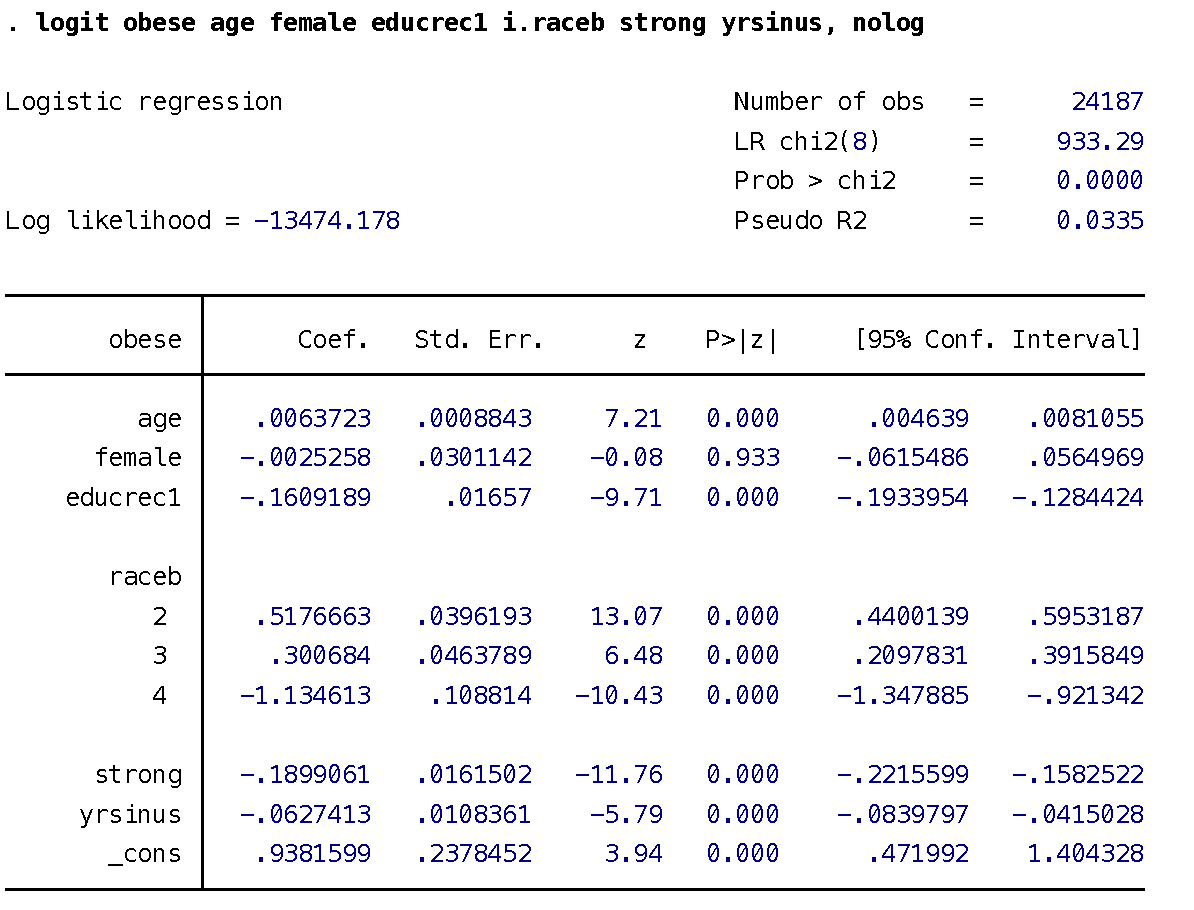
\includegraphics[scale=.5]{images/obese_logit.pdf}
% 
%       \caption[Standard \cmd{logit} output (1): Log odds coefficients]{\label{tbl:logit}
%     Standard \cmd{logit} output (1): Log odds coefficients.\\
%     \nhis{24,187}}
%   \end{table}%
% 
%   The coefficients of a logistic regression are radically different to those of a linear model. The \emph{link function} that underlies the model does not take the form $Y = \alpha + \beta X$ but instead define the log-likelihood of $Y$, where the likelihood of $Y$ is the sum of its `successes' $Pr(Y=1)=p$ divided by the sum of its `failures' $Pr(Y=0)=1-p$. The ratio $p/(1-p)$ is then transformed to its natural logarithm, in order to escape the 0--1 bounds of the probability $p$ and obtain regression coefficients as \emph{log odds}, which can range from 0 to infinity, and which basically measure the magnitude of each independent variable as a probabilistic predictor of $Y$.
%   
%   In a logistic model, just as with linear regression, the constant is the null estimator, or $Pr(Y=1)=\alpha$ when all other variables are held constant. The constant indicates that the models `starts' with a probability of being obese of $exp(.94)/(1-exp(.94))=.71$, or 71\%.\footnote{You can ask Stata to display that result, with the \cmd{di}{display} command: \texttt{di exp(.94)/(1-exp(.94))} (turn to \statacode{help math functions} for more math equation fun).} This probability is then enhanced by positive coefficients or penalized by negative ones, proportionally to their estimated values. In this model, race increases the log odds of being obese for individuals in the categories 2 (Blacks) and 3 (Hispanics); reversely, the negative log odds of the fourth race group (Asians) indicates a reduced risk of obesity. Similarly, every year of education above Grade 12 also predicts a lesser likelihood of being obese: for each increase in \texttt{educrec1}, a measure of educational attainment, the odds of being obese drop by $exp(-.16)/(1-exp(-.16))=.46$, or 46\%.
% 
%   % [todo: expand on OR] http://www.theanalysisfactor.com/why-use-odds-ratios/
%   
%   Table~\ref{tbl:logodds} shows how \emph{odds ratios}\index{Odds ratios!Logistic regression}\index{Odds ratios|seealso{Logistic regression}} offer to read logistic coefficients, by taking the exponents $e^\beta$ of the log odds. The \opt{or}{logit} option replaces log odds with odds ratios in a \cmd{logit} output. These ratios read as increases in proportions: in this model, the risk of obesity is 67\% \ie two thirds higher among Blacks than it is among Whites. Odds ratios inferior to 1 denote, on the contrary, a reduction in likelihood, as with Asians, who are $.32$  \ie one third \emph{less} likely to be obese than Whites.
% 
%   \begin{table}[htp]
%     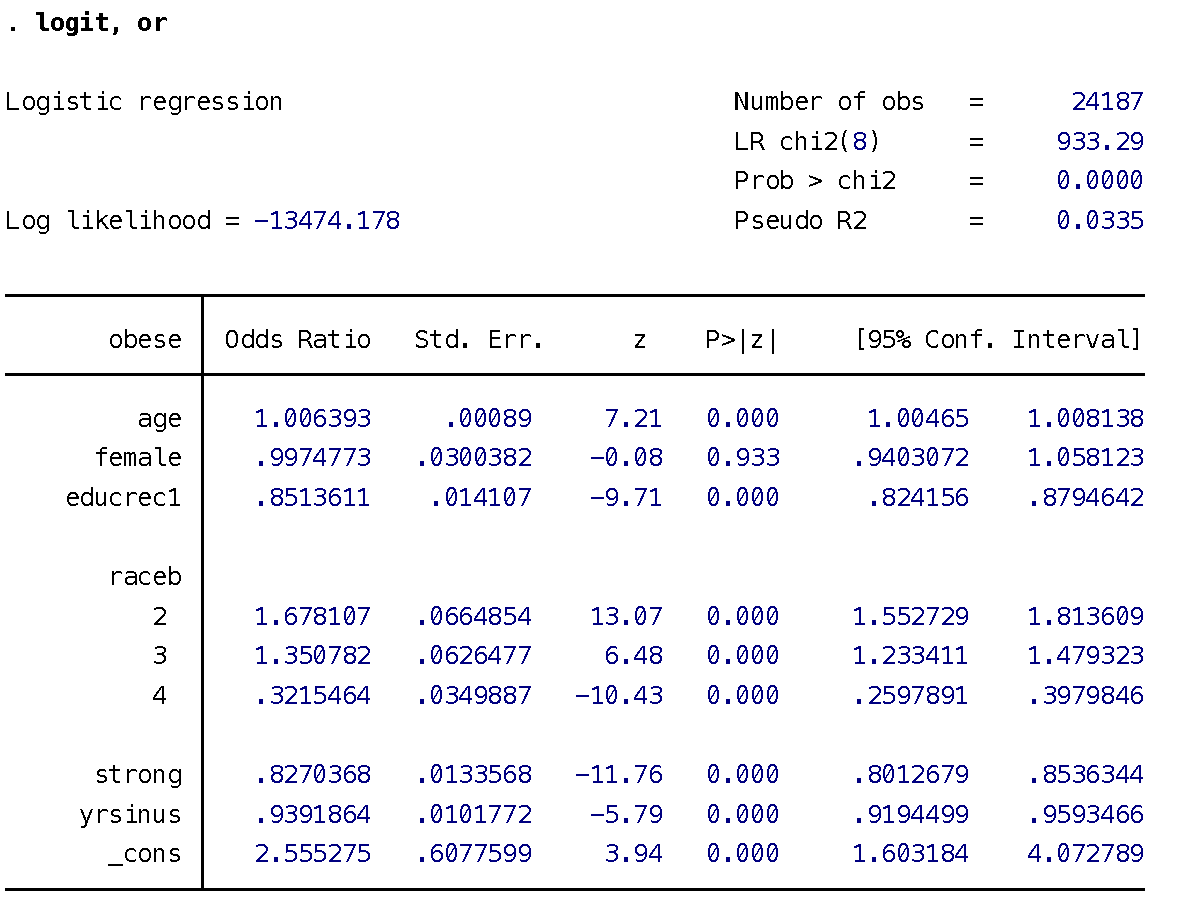
\includegraphics[scale=.5]{images/obese_logodds.pdf}
% 
%       \caption[Standard \cmd{logit} output (2): Odds ratios]{\label{tbl:logodds}
%     Standard \cmd{logit} output (2): Odds ratios (shown with the \opt{or}{logit} option).\\
%     \nhis{24,187}}
%   \end{table}%
% 
%   Table~\ref{tbl:wald} shows how you can further measure the probability that two coefficients are simultaneously significant by performing a Wald significance test with the \cmd{test} command\index{Significance tests!Wald test}. In this example, the coefficients for Blacks and Hispanics are shown to be both significantly different from the null hypothesis. Using a Wald test that fits your theoretical insights is arguably a better method of validation for your model than looking at its overall fit, which is not as easy to measure or interpret in nonlinear models.
%   
%   \begin{table}[htp]
%     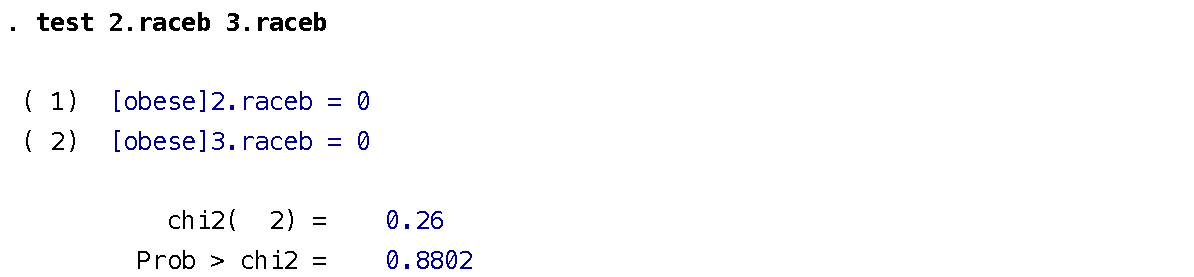
\includegraphics[scale=.5]{images/obese_wald.pdf}
% 
%       \caption[Wald significance test on logistic regression coefficients]{\label{tbl:wald}
%     Wald significance test on logistic regression coefficients.\\
%     \nhis{24,187}}
%   \end{table}%
% 
%   Table~\ref{tbl:obese_aic_bic} shows a comparison of two models, displayed with \cmd{estout}. The $R^2$ is a pseudo-measurement in a logistic regression model that hardly reflects the actual fit of the model, even in refined measurements like McKelvey and Zavoina's $R^2$. Some researchers will use AIC and BIC, two criteria with slightly different assumptions but that should converge in most cases, with higher values indicating better fit, as is the case here when race and education are considered. Fit statistics for logistic models, however, are not that useful overall.
% 
%   \begin{table}[htp]
%     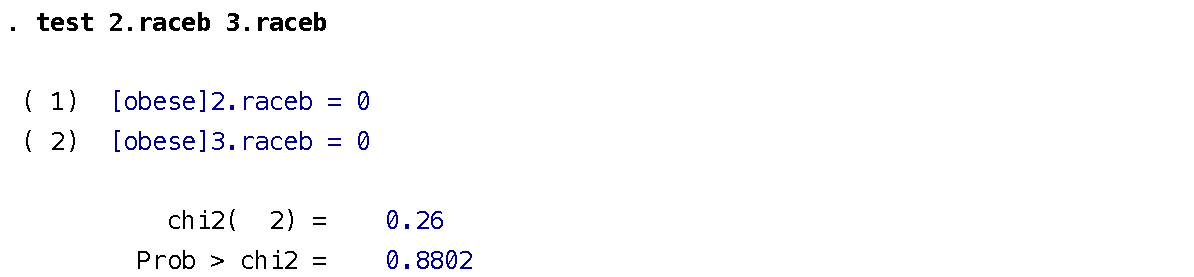
\includegraphics[scale=.5]{images/obese_wald.pdf}
% 
%       \caption[Fit statistics in \cmd{estout} output for \cmd{logit} models]{\label{tbl:obese_aic_bic}
%     Fit statistics in \cmd{estout} output for \cmd{logit} models. See \statacode{help estout} and related online documentation for options.\\
%     \nhis{24,187}}
%   \end{table}%
% 
%   Table~\ref{tbl:ologit} shows that, just as with linear regression, the output of logistic regression in Stata can be simplified with the \cmd{leanout} command, first shown at p.~\pageref{sec:leanout}. The model is an \emph{ordinal logit}, where the dependent variable comes in ordered categories for which the numerical interval makes little sense: here, for instance, being underweight is coded as `1' and obesity is coded as `3', but it makes no sense to consider that being obese is like being three times underweight, or that being normal is to be `2' right in the middle.\index{Data!Ordinal data} Ordinal models come with \emph{cut points} that define the probability level of each category, which provide additional information to assess the likelihood of each category of the dependent variable.\footnote{Stata uses a specific notation for ordinal results: \url{http://www.stata.com/support/faqs/stat/oprobit.html}.}
% 
%   \begin{table}[htp]
%     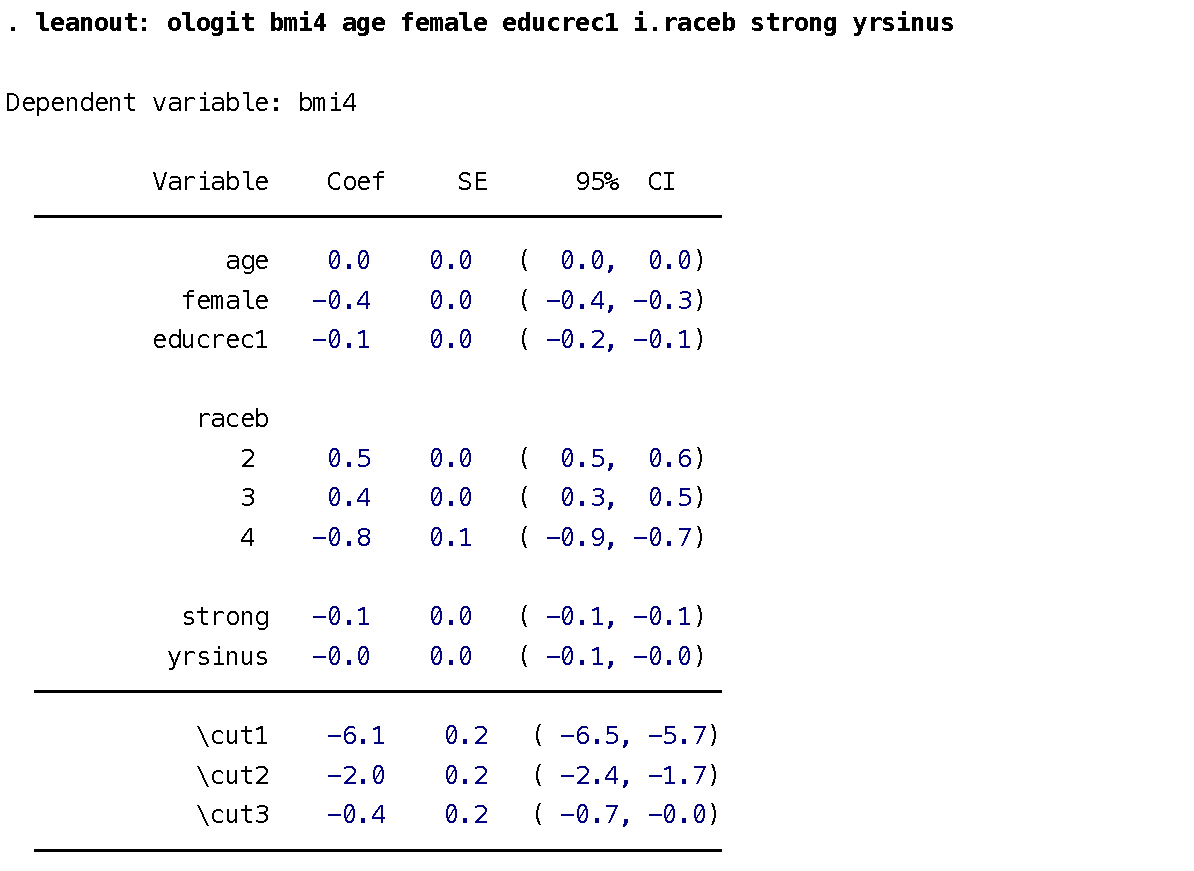
\includegraphics[scale=.5]{images/obese_ologit.pdf}
% 
%       \caption[Fit statistics in \cmd{estout} output for \cmd{logit} models]{\label{tbl:ologit}
%     Ordinal logit model estimated with \cmd{ologit} and processed with \cmd{leanout}. See \statacode{help estout} and related online documentation for options.\\
%     \nhis{24,187}}
%   \end{table}%
%   
%    Figure~\ref{fig:diabetic_95ci} finally shows how logistic models can be simulated with the commands of the \cmd{clarify} package, previously mentioned at p.~\pageref{sec:sim}. These commands allow to estimate the effects attributable to a single predictor by holding other variables constant, while setting a clear `starting point' to the simulation. The figure shows how five years of education set apart American adults in their risk of becoming diabetic: throughout the life course, the probability level $Pr(\text{diabetic}=1)$ ends up being approximately twice as large at low versus high levels of education, independently of all other factors included in the model.
% 
%   \begin{figure}[htp]
%     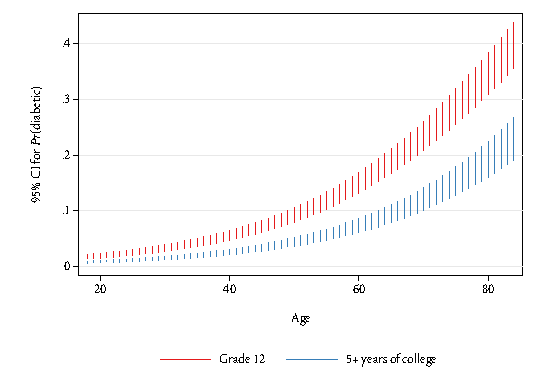
\includegraphics[width=.9\textwidth]{images/diabetic_95ci.pdf}
% 
%     \caption[Simulated probabilities of diabetes by age and education]{\label{fig:diabetic_95ci}
%     Simulated probabilities of diabetes by age and education. Code adapted from the replication material for \cite{KingTomz:2000a}.\\
%     \nhis{24,187} (1,000 simulations)}
%   \end{figure}%
% 
%   Plotting the marginal effects or odds ratios of logistic models can be done in various ways, and regression diagnostics also exist for all the models mentioned above. There are also many applications of count models in health and social sciences. The overall diversity of regression models is one of its strengths as a method of analysis, as it indicates careful attention to the background assumptions that go into statistical analysis; the drawback, of course, is that model selection can become quite difficult and erratic.
% 
%   \paragraph{Time series}%
%   \label{sec:ts}\index{Data!Times series}\index{Time series|see{Data}}%
%   %
%   Time series hold unique observations for $N$ units at $\bar T = 1, \ldots, t$ temporal units, usually years or quarters. It contrasts with longitudinal panel data because it often aims at forecasting the forthcoming values of the series, rather than simply clustering them to reduce the standard error of the model. Time series are also helpful for analyzing the probability of occurrence of recurrence of some historical events, which can apply to a broad range of subjects and has tons of interesting applications in the social sciences.\footcite{Box-SteffensmeierJones:2004b}
% 
%   Stata understands that the data are time series once you pass it a few parameters about your $t$ variable and its format with the \cmd{tsset} command. You would then have to check the properties of your time series, such as stationarity or autocorrelation, in order to set up an appropriate model for your series. A large class of these models are said to be autoregressive, as they primarily rely on the past values of $X$ ($X_{t-1}, X_{t-2}, \ldots, X_{t-k}$) to linearly infer its more recent values.
%   
%   The methods of time series analysis use differentiation to analyze significant variations in the current series, and simulations to identify the confidence interval for future values. These methods have important applications for country-level data because cross-sectional times series often underemphasize the substantive significance of autocorrelation, which can closely reflect the notion of  ``institutional stickiness'' and related concepts. This use of time series analysis would greatly benefit to comparative politics and other fields of inquiry where path dependence and feedback effects are determinant.
% 
%   %
%   %
%   %
%   \paragraph{Bayesian statistics}%
%   %
%   \index{Bayesian \emph{versus} frequentist statistics}%
%   \label{sec:bayesian}
%   %
%   \emph{Bayesian data analysis} uses Bayes' Theorem to promote another understanding of probability than the one promoted by the Central Limit Theorem and \emph{frequentist} statistics. Instead of relying on normally distributed probabilities, it injects subjective probabilities into the model, in order to reflect prior information accessible to the subjects modeled by the estimator. This approach is quite relevant to social science subjects, given that units of observation like households, governments or companies can be expected to use such information in the formation of their preferences. This approach is also relevant to account for bias in addition to strategic behavior, which eventually makes it very appropriate in many social contexts. Most approaches to multilevel models will introduce you to Bayesian statistics.\footcite[For a book-length introduction with R code, see][but get a serious grip at frequentist statistics first.]{GelmanHill:2007a}

%
%
%
\section{Interpretation}

We will use a breakdown of Table~\ref{tbl:hibbs_yx1_regress} to explain standard Stata output for the \cmmd{reg} command, which estimates the simple linear regression model \texttt{reg bread vote}. You should read your model by looking briefly at the \emph{goodness of fit} of the model, and then focus on understanding the \emph{regression coefficients}.

% \begin{table}[htp]
% 	\begin{itemize}
% 		\item \emph{Analysis of variance} (left) and \emph{goodness of fit} (right):\\
% 		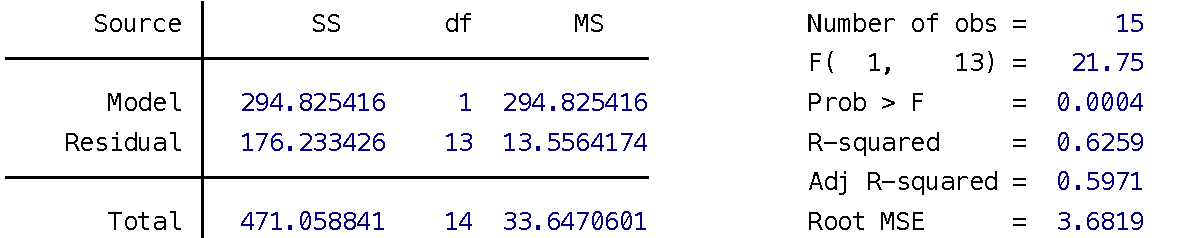
\includegraphics[scale=.5]{figures/hibbs_yx1_regress_top.pdf}
% 	
% 		\item \emph{Regression coefficients}, including constant (\texttt{\_cons}):\\
% 		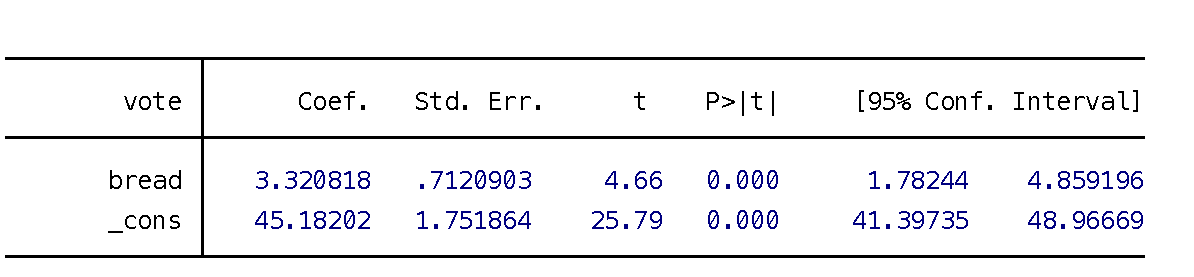
\includegraphics[scale=.5]{figures/hibbs_yx1_regress_bottom.pdf}
% 	\end{itemize}
% 
% 	\caption[Breakdown of regression output with \cmmd{reg}]{\label{tbl:hibbs_yx1_regbits}
% 	Breakdown of regression output with \cmmd{reg}.\\
% 	\hibbs{15}}
% \end{table}%

	%
	% 6.1.1
	%
	\subsection{Goodness of fit}

	\label{sec:goodness}%
	%
	Table~\ref{tbl:regression_fit} shows the variance table (left), which details the sum of squares for the model and for its residuals. This information is redundant with an analysis of variance, and is used to derive information on the goodness of fit (right):

	\begin{table}[htp]
		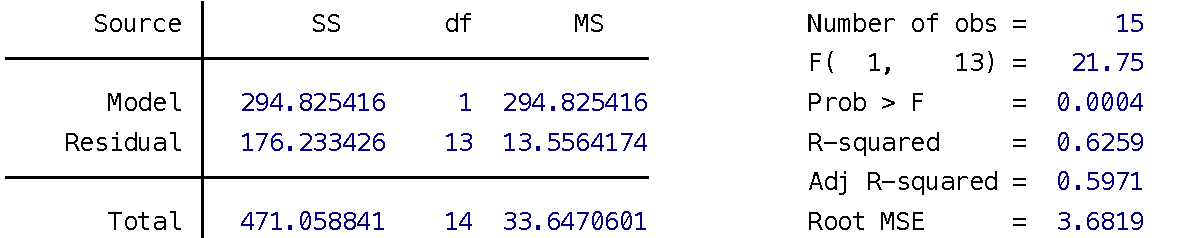
\includegraphics[scale=.5]{figures/hibbs_yx1_regress_top.pdf}

	  	\caption[Extract from \cmmd{reg} output (1): Variance and goodness of fit]{\label{tbl:regression_fit}
		Extract from \cmmd{reg} output (1): Variance and goodness of fit.\\
		\hibbs{15}}
	\end{table}%

	\begin{itemize}
		\item The \textbf{number of observations} constrains your whole model: all statistical results are derived from and only from the set of observations included in the linear regression, after listwise deletion (explained on p.~\pageref{casewise}). The model cannot be more intelligent than this set of observation: only you can. If a large fraction of the data is not represented in the analysis, you will have to describe the subset on which you are running your analysis, and assess to what extent you can generalize its results.

		\item The \textbf{$F$-statistic} is used to test whether your model is significantly different from the null estimator $H_0: \beta = 0 \Rightarrow \beta X = 0 \Rightarrow Y = \alpha$. In other words, it tests whether the regression line of your model is `flat' and equivalent to the mean value of $Y$ in its ability to describe its distribution. This is the null hypothesis of regression overall, and is also used for each coefficient in the model. The substantive significance of your model will rarely need to verify this hypothesis.\footnote{This means that, in theory, there is no real grounds to be concerned about the $p$-value of the $F$-test. What happens in practice is that multiple regression models quickly become statistically significant.}
		
		\item The \textbf{$R^2$ (R-squared)} is the ratio of predicted variance, $\sum{(\hat{Y_i}-\bar{Y_i})^2}$, by the total variance in the data, $\sum{(Y_i-\bar{Y_i})^2}$, for $i=1, \ldots, n$ observations. As the unpredicted variance (RSS) approaches 0, the $R^2$ will approach 1, which makes it simple to understand. The adjusted $R^2$ corrects for factors that artificially inflate the statistic.\footnote{There is a wealth of other measures that penalize even more the predicted variance, to obtain more conservative estimates of how much is actually predicted. For social science data, this game is generally not so relevant.} In the present example, the `Bread and Peace' model therefore predicts around 60\% of the variance in presidential votes on 15 postwar elections, which is statistically remarkable.
		
		The substantive significance of the $R^2$ is limited: it is perfectly justifiable to research an association that does not efficiently minimizes unpredicted variance. You should, however, use it to compare the predictive exhaustiveness of several models. Table~\ref{tbl:hibbs_yx1_estout} provided an example of such a comparison: the `Bread and Peace' model, which is already highly efficient over all election years ($R^2\approx.6$), can become even more efficient without election years affected by war ($R^2\approx.8$). In a multiple regression, you might also want to try out several models to compare how much your model changes in absence or presence of a single variable.

		% http://www.theanalysisfactor.com/small-r-squared/

		\item\label{rmse_explained} The \textbf{Root MSE} (Root Mean Square Error) is the RMSE briefly mentioned at p.~\pageref{rmse}, and is another way to understand the error term of the model. The RMSE is measured in the same units as the dependent variable $Y$ and indicates the mean distance between fitted and actual data points. In the present example, the `Bread and Peace' model is therefore, on average, three percentage points wrong about the actual presidential vote. This measure is meaningful only if you can interpret it: in the case of a presidential election, three percentage points is a meaningful margin of error.

	\end{itemize}

	%
	% 6.1.2
	%
  % unstd, std, dummies
  %
	\subsection{Regression coefficients}
	\paragraph{Interpreting coefficients}%
	\label{sec:coefficients}%
	%
	Table~\ref{tbl:regression_coef} shows the regression coefficients and related information, which is the heart of the model. Whether your model is statistically significant or whether it captures a large fraction of variance is of limited importance in comparison to the coefficient estimates of the regressors. A statistically insignificant model, for instance, will fail to estimate a single reliable predictor. In practical terms, this implies you need not spend more than a minute on the goodness of fit of your model, and should instead pay \emph{more than careful} attention to its coefficients:

	\begin{table}[htp]
		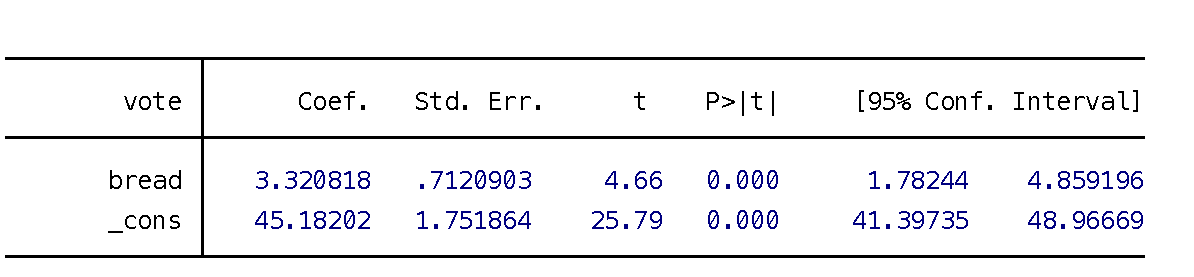
\includegraphics[scale=.5]{figures/hibbs_yx1_regress_bottom.pdf}

	  	\caption[Extract from \cmmd{reg} output (2): Regression coefficients]{\label{tbl:regression_coef}
		Extract from \cmmd{reg} output (2): Regression coefficients.\\
		\hibbs{15}}
	\end{table}%

	The coefficients, or regression \emph{parameters}, were estimated through \emph{maximum likelihood}\index{Models!Maximum Likelihood Estimation (MLE)}, a method of estimation that can be used with several regression models.\footnote{Maximum likelihood estimation (MLE) is also used for logistic regression, which is briefly described and illustrated at p.~\pageref{sec:logit}.} What they intend to measure, beyond the statistical significance of the independent variable $X$ for predicting the dependent variable $Y$, is its \emph{marginal effect}\index{Linear regression!Marginal effects}\index{Marginal effects|seealso{Linear regression}}: as in the linear function $Y=\beta X$, when $X$ increases by one unit, $Y$ increases by $\beta$ units, where $\beta$ is the regression coefficient of $X$. If the coefficient is negative, then $Y$ decreases by $\beta$ units when $X$ increases by one unit.

	In the present example, the model `starts' at the constant, $\alpha \approx 45.18$, which is the level of presidential support $\bar Y$ predicted by the model when the \texttt{bread} parameter is null (or, in quick notation, $\alpha = E(Y|X=0)$). This constant is theoretical and not always as meaningful as it is here. This is because from that point, the model predicts that every increase in one unit of the \texttt{bread} variable (real growth in disposable income, in \%) is associated to an increase in $\beta \approx 3.32$. Linear regression is an additive model, and the regression parameter is positive, which is why it makes sense to describe the model as an engine that estimates `constant' presidential support around 45\%, and then predicts a `marginal' increase of 3.3 percentage points in support for each percentage point of real disposable income growth.
	
	Table~\ref{tbl:hibbs_yx1x2} illustrates how this rule of calculation stays true when you add variables to perform \emph{multiple linear regression}. Regression coefficients are estimated for each variable while holding all other variables constant at zero value. For that reason, they are ceteris paribus measures that capture the effect of each variable ``all things equal'' i.e. all other model variables held at a constant value of nil. In our example, the addition of the \texttt{death} variable to the model shows that every U.S. fatality per million population reduces presidential support by $\beta_2 X_2=-.05$. This effect is a `net' effect, \emph{independent} of the economic circumstances captured by the \texttt{bread} variable. In parallel, the positive effect of income growth on presidential support is verified while \emph{controlling for} the effect of military fatalities.

	\begin{table}[htp]
		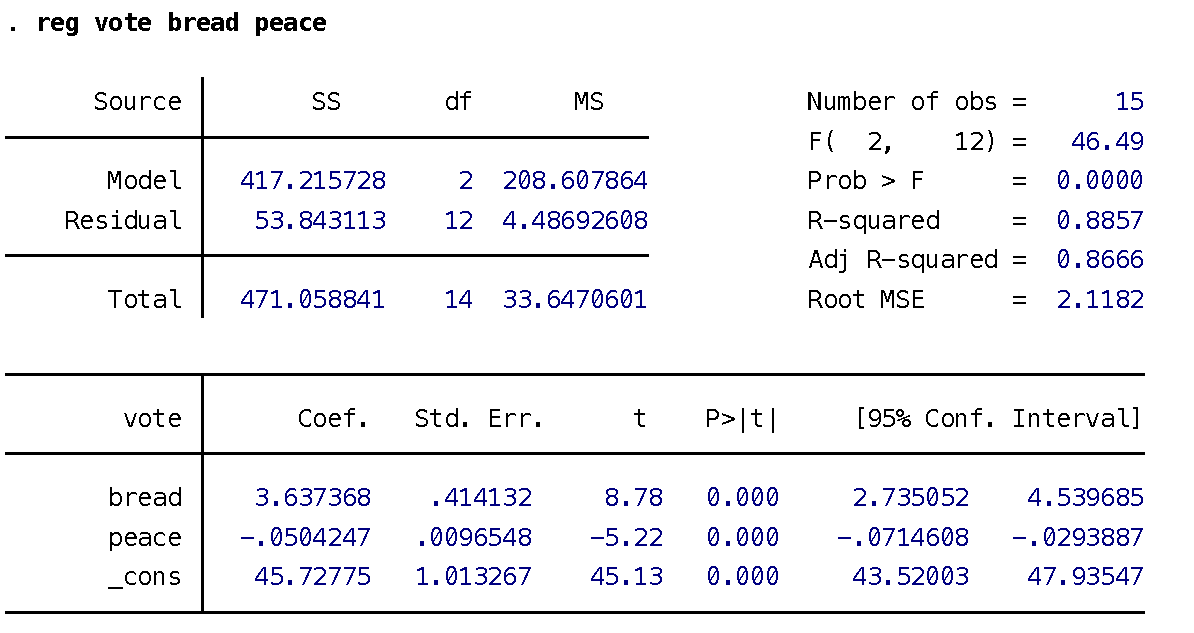
\includegraphics[scale=.5]{figures/hibbs_yx1x2.pdf}

	  	\caption[Extract from \cmmd{reg} output (3): Multiple regression coefficients]{\label{tbl:hibbs_yx1x2}
		Extract from \cmmd{reg} output (3): Multiple regression coefficients.\\
		\hibbs{15}}
	\end{table}%
	
	Any model that yields one statistically significant coefficient can be interesting to interpret, but make sure that you read regression coefficients within their confidence bounds: standard errors can be quite large in low-$N$ samples, and their confidence intervals can be consequently large too, as is the case here in the `Bread and Peace' model. Stata displays the standard errors and the ratio between the coefficient and its standard error, the $t$-value, which is used to compute the $p$-value from the $t$-distribution. If the confidence interval of your coefficient comes close to include zero, then its marginal effect might well be null or close to null.
	
	To assess whether you know enough about the coefficients of your model, try fitting a real value of $Y$. For example, in the simplified `Bread and Peace' model that is presented here, a stable income growth of $X_1=2$ percentage points with a low number of $X_2=50$ war casualties per million population leads to a predicted electoral support of $\hat Y = 45.7 + 2*3.6 + 50*(-.05) \approx 50.4\%$ in favor of the incumbent president.

	\paragraph{Dummies}%
	\label{sec:dummies}%
	%
	Dummies are a way to measure a dichotomous condition, such as being female (1) or non-female (0), White (1) or non-White (0), etc. The parametric estimate of a dummy variable is the independent effect of that condition when it is verified in the data. In the regression equation, a dummy is just a true/false condition for a coefficient, as in this example equation that compares the value of a dependent variable $Y$ in democracies versus dictatorships:

	\[
	  Y = \alpha + \beta_1 X_1 + \beta_2 X_2 + {\color{red}\beta_3 \times \text{democracy}} \left\{ 
	  \begin{array}{l l}
	    \text{if~democracy}=0 \\ \quad Y = \alpha + \beta_1 X_1 + \beta_2 X_2 + \beta_3 \times 0\\[1em]
	    \text{if~democracy}=1 \\ \quad Y = \alpha + \beta_1 X_1 + \beta_2 X_2 + \color{red}\beta_3 \times 1\\
	  \end{array}\right\}
	\]
	
	In this equation, the \texttt{democracy} coefficient is not estimated for dictatorships, which means that the dictatorship category is the \emph{reference category}, or the \emph{baseline} of your model. The \texttt{democracy} coefficient $\beta 3$ in the regression represents the \emph{net effect} on this baseline. You can code any categorical variable as one or more dummies with either \cmmd{recode} or \abbr{tab}{tabulate} with the \texttt{gen(dummy)} option, and therefore calculate the net effect of each categorical predictor.

	Table~\ref{tbl:abortion_dummy} shows a practical example of a dummy coding for democratic regimes in a multiple linear regression at the country level. The dummy is preceded by the \abbr{i.}{interaction} prefix command. The coefficient for the \texttt{1.democracy} variable indicates how the dependent variable compares in democracies versus dictatorships when holding all other variables in the model constant. The coefficient is positive, indicating that on average, democracies enjoy higher support for abortion; the standard error on that estimate, however, is too high, and the coefficient is statistically insignificant.

	In that same regression table, another categorical variable codes for political regime: \texttt{dpi\_system} distinguishes presidential, parliamentary and mixed regimes. In the \texttt{dpi\_system} variable, presidential regimes were coded \texttt{0} and are the reference category. The overall model therefore uses dictatorial presidential regimes to measure whether support for abortion is higher or lower in other regimes, the results of which are the dummy coefficients. In this example, the only statistically significant category codes for parliamentary regimes (\texttt{dpi\_system~==~2}).

	\begin{table}[htp]
		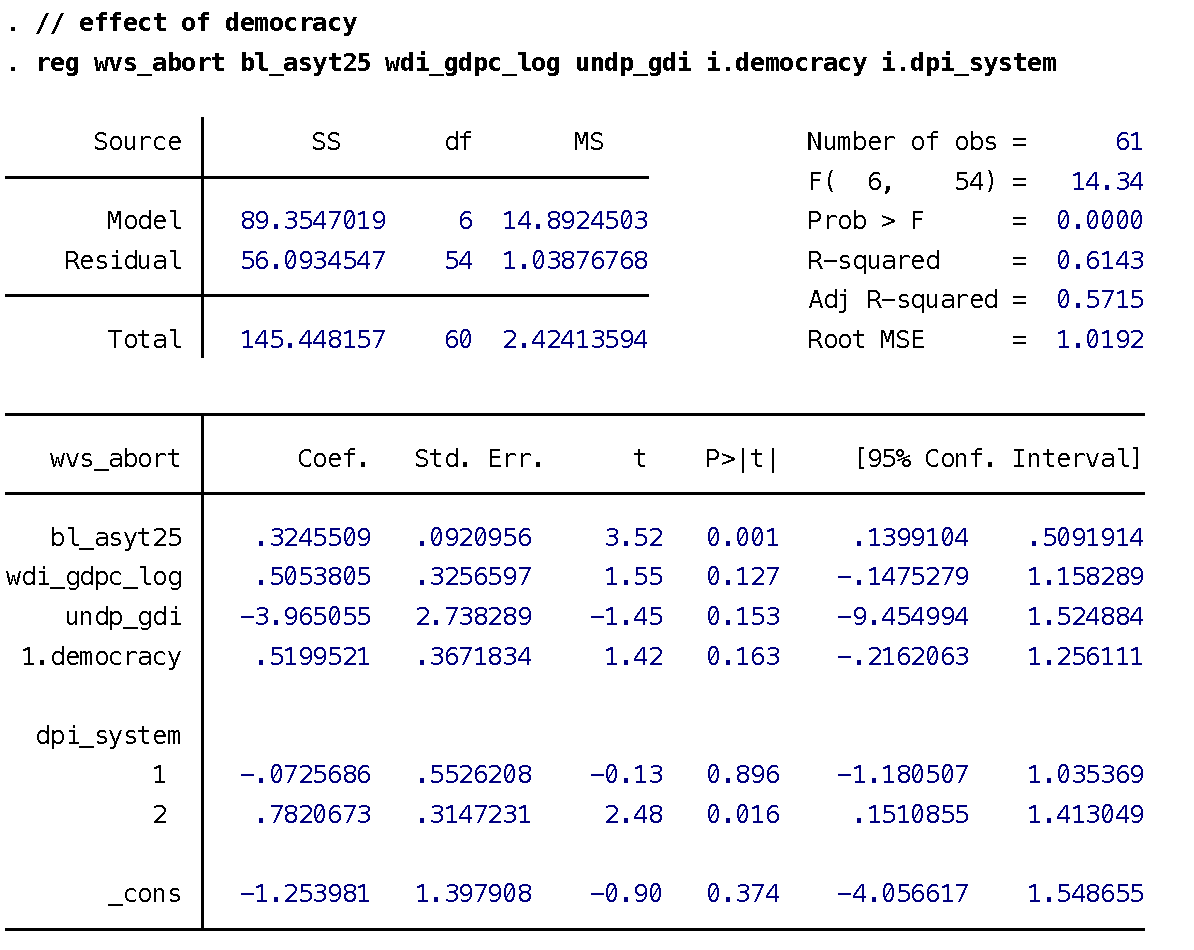
\includegraphics[scale=.5]{figures/abortion_dummy.pdf}

	  	\caption[Linear regression with a dummy]{\label{tbl:abortion_dummy}
		Linear regression with the \texttt{i.democracy} dummy, recoded from variable \texttt{gol\_polreg}.\\
		\qog{61}}
	\end{table}%
	
	Figure~\ref{fig:abortion_dummy_plot} shows how this dummy translates graphically: democracies and dictatorships have been estimated in the same way, using the same variables with the same coefficients. However, the regression line for democracies (red) is slightly above the baseline model for dictatorships (blue). The distance between the two parallel regression lines is the (positive) net effect of \texttt{i.democracy} on the dependent variable \texttt{wvs\_abort}. This effect is rather minor, since many other predictors are also correlated to democracy and absorb most of its variance.

	\begin{figure}[htp]
		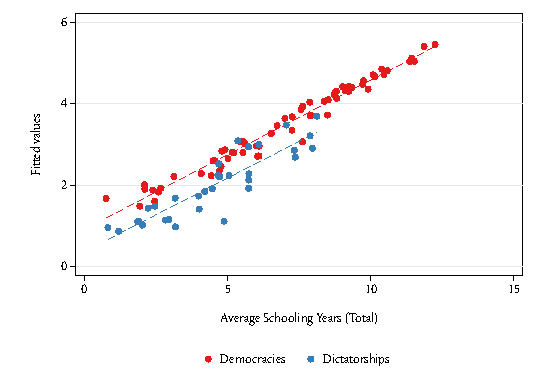
\includegraphics[width=.9\textwidth]{figures/abortion_dummy_plot.pdf}

		\caption[Plotting the effect of a dummy]{\label{fig:abortion_dummy_plot}
		Plotting the effect of the \texttt{i.democracy} dummy with two linear fits of Table~\ref{tbl:abortion_dummy}.\\
		\qog{61}}
	\end{figure}%

	Stata will accept the \abbr{i.}{interaction} prefix command in front of any categorical variable, and will select the first category as the baseline. Dummies are simple to implement but are useful \emph{only once you know the baseline of the model}. If you are coding a lot of information as dummies, then your model describes a theoretical `zero' situation where all dummies are equal to nil. Since you have to interpret dummies in reference to that situation, make sure that you understand what is the reference category of each dummy.

	% http://www.theanalysisfactor.com/confusing-statistical-term-6-factor/
  
	\paragraph{Standardized coefficients with \copt{beta}{regress}}%
	\label{sec:beta}%
	%
	Your coefficients can be interpreted in more than metric form. It might well be, for instance, that your variables have been transformed in such as way, or measured in such units, that metric coefficients will make little sense even when statistically significant. The fundamental problem lies with the units of your coefficients, which are dependent on the units of measurement of your variables. For example, given that education and income have different units, you cannot compare the effect of education (which the coefficient measures in years of schooling) and income (which the coefficient measures in constant dollars). Identically, the `Bread' and `Peace' variables are calculated on different units of different distributions.
	
	Table~\ref{tbl:hibbs_yx1x2_beta} shows how to solve that issue with standardized, a.k.a `beta' coefficients. These coefficients are measured from a standardized measure of each $Y$ and $X$ variable, and therefore share the same units. When you add the \copt{beta}{regress} option to the \cmmd{reg} command, these coefficients replace the confidence intervals in the Stata output.

	\begin{table}[htp]
		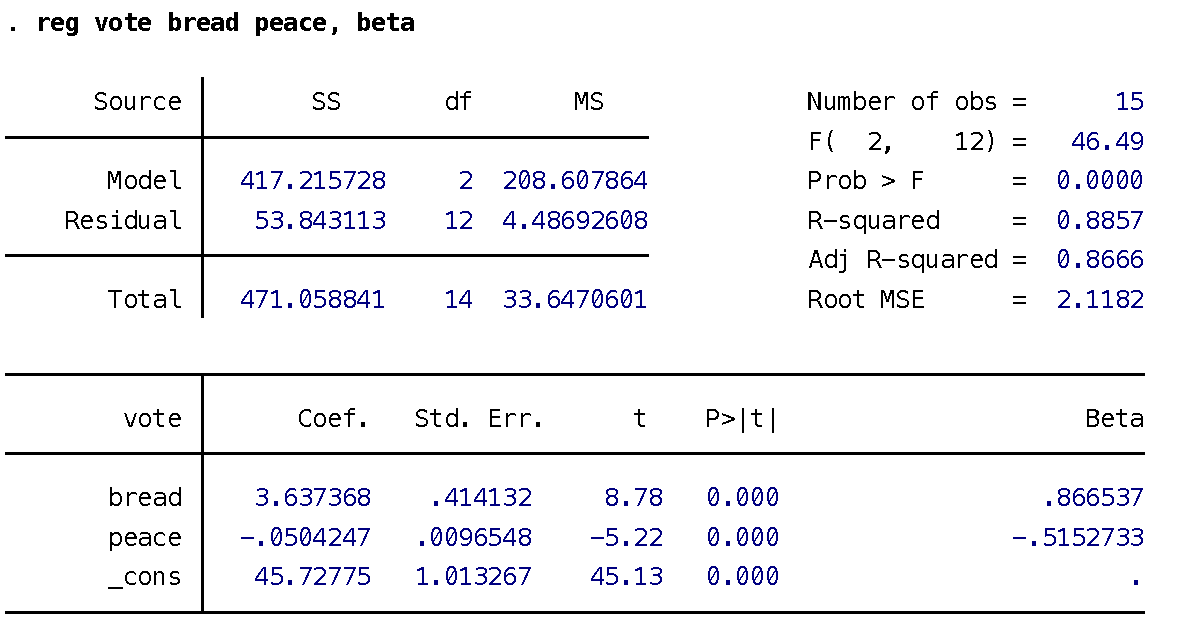
\includegraphics[scale=.5]{figures/hibbs_yx1x2_beta.pdf}

	  	\caption[Extract from \cmmd{reg} output (5): Standardized regression coefficients]{\label{tbl:hibbs_yx1x2_beta}
		Extract from \cmmd{reg} output (5): Standardized regression coefficients.\\
		\hibbs{15}}
	\end{table}%
	
	Standardized coefficients should be read as an approximate measure of \emph{statistical} influence: the more variance a variable captures, the further away from zero its standardized coefficient will be. The positive or negative sign does not apply to the magnitude of standardized coefficients, only their `distance' to zero. This is not a measure of substantive influence or even less causal influence by any means. However, it gives you a hierarchy of importance that shows, for example, that the `Bread and Peace' model is primordially driven by the \texttt{bread} (economy) variable, whose standard coefficient is close to .8, while the peace variable carries less statistical weight with an \emph{absolute} standardized coefficient of .51.
  
	%
	% 6.1.3
	%
	\subsection{Exporting results}

  % leanout
  % estout
  % plotbeta (?)

\paragraph{Exporting with \cmmd{estout}}%
  \index{Linear regression!Storing estimates}%

Table~\ref{tbl:hibbs_yx1_estout}, finally, shows a few more commands to format your results straight away for storage and export with the \cmmd{estout} package. The \cmmd{eststo} command stores the estimates of any number of models, and the \cmmd{esttab} command allows selecting only part of the regression output, for viewing and/or exporting purposes.

\begin{table}[htp]
	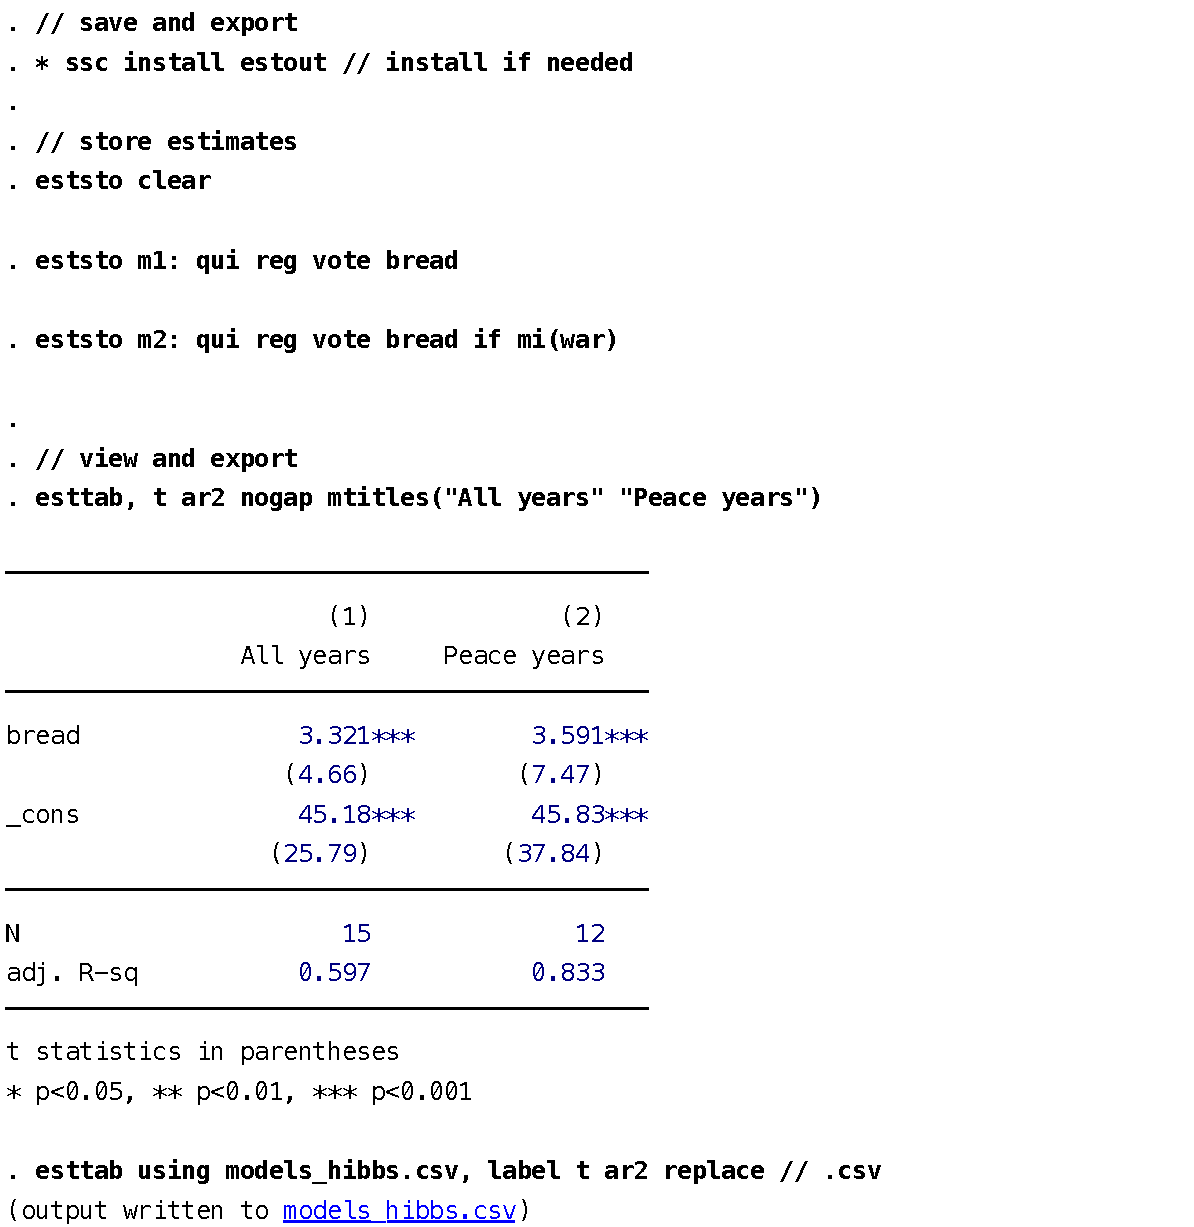
\includegraphics[scale=.5]{figures/hibbs_yx1_estout.pdf}

	\caption[Storing estimates with \cmmd{predict}]{\label{tbl:hibbs_yx1_estout}
	Storing and exporting estimates with \cmmd{estout}.\\
	See \texttt{help estout} and related online documentation for options. \emph{Note:} the \cmmd{reg} command is muted by the \abbr{qui}{quietly} command in this code; its output does not show up on screen, but the command ran `silently' in the background. \hibbs{12-15}}
\end{table}%

\paragraph{Formatting instructions} See Table~\ref{tbl:estout_reg} at p.~\pageref{tbl:estout_reg} for layout instructions and code.

The \cmmd{estout} package is very flexible. The example shown uses only $t$-statistics (option \texttt{t}) and adjusted $R^2$ (option \texttt{ar2}), but you can cook different output with standard errors (option \texttt{se}) and standardized coefficients (option \copt{beta}{esttab}), depending on your preferred method of reading. The next section explains how each of these elements inform the model.

Finally, note that the code used with the \cmmd{estout} command actually estimates \emph{two} models: `Model 1' was estimated on all elections years ($N=15$), while `Model 2' was estimated only on $N=12$ elections years for which military fatalities were not a significant factor. The estimates can be compared between models, which we will also illustrate below.

	
	\paragraph{Simplifying interpretation with \cmmd{leanout}}%
	\label{sec:leanout}
	%
	The \cmmd{leanout} package is a prefix command that reduces regression output to a minimum, so that you can concentrate on the essentials. The \texttt{estout} package already introduced that logic: Table~\ref{tbl:hibbs_yx1_estout} at p.~\pageref{tbl:hibbs_yx1_estout} showed only a few statistics in comparison to the standard Stata output, with much less precision to better represent the true level of accuracy in social science data. The output of the \cmmd{leanout} command is also ``rather draconian'' and loses all information related to the $t$-tests, focusing instead on the actual values of the coefficients and their standard errors.\footcite{Beck:2011a}

	Table~\ref{tbl:hibbs_yx1x2_leanout} shows \cmmd{leanout} syntax and output. Again like \cmmd{estout} command, the \cmmd{leanout} command is a prefix to the \texttt{reg} command (and to other regression commands).
	
	\begin{table}[htp]
		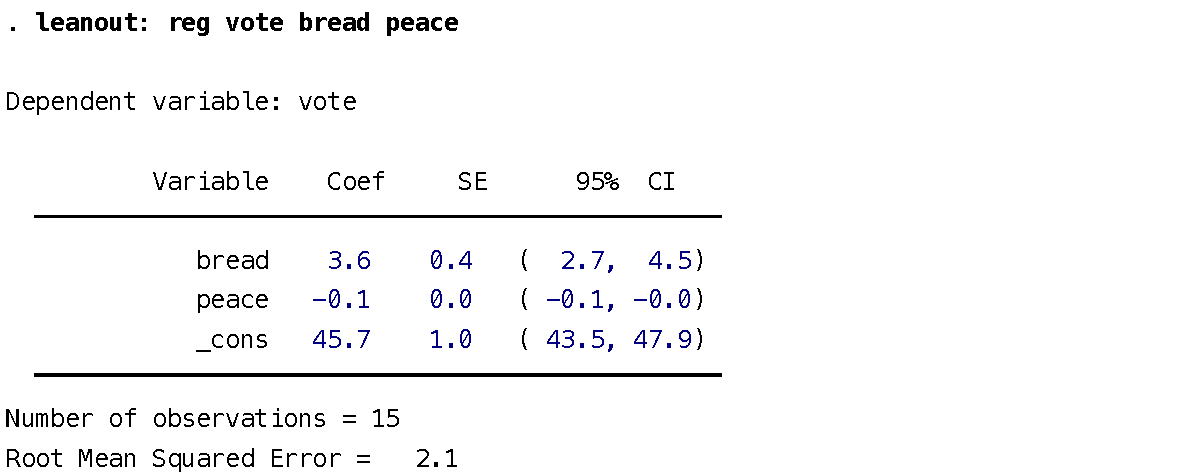
\includegraphics[scale=.5]{figures/hibbs_yx1x2_leanout.pdf}

	  	\caption[Extract from \cmmd{reg} output (4): Simplified regression output]{\label{tbl:hibbs_yx1x2_leanout}
		Extract from \cmmd{reg} output (4): Simplified regression output using the \cmmd{leanout} prefix.\\
		\hibbs{15}}
	\end{table}%
	
	The drastic reduction of information obtained through \cmmd{leanout} is a good exercise in itself to check whether you understand regression coefficients correctly. The parameters selected by \cmmd{leanout} are expressed in real-world units, which encourages the reader to read standard errors, confidence intervals and the RMSE rather than $p$-values. This approach makes sense, especially when interpreting unstandardized coefficients for untransformed variables, because in that case, you are able to read coefficients in the same metric as the actual variables, such as years, currencies, percentage points or counts (i.e. numbers of something: alcoholic beverages per week, sexual partners in the last five years, whatever).

	%If you find it difficult to interpret coefficients without their significance tests with $t$-values and $p$-values, then you are experiencing exactly what any conventional quantitative social researcher would experience in the same situation.
	Frequentist statistics, like linear regression analysis, insist heavily on measuring the probability level of the null hypothesis. The interpretation of $p$-values, however, is substantively limited: a $p$-value does not indicate the strength of an association, and it does not translate as the chance of a significant association.\footnote{Even when Stata displays a probability level as `\texttt{Pr = 0.000},' it really means that $p < .0001$.}
	
	If you are on your way to analyze the data \emph{metrically}, which is a best-case scenario, then \cmmd{leanout} will force you to consider the confidence bounds of your parameters and the proximity of the whole confidence interval to zero. In absence of a `star system' and $p$-values, you are also forced to consider the actual value of the standard errors. Intellectually, the end process is equivalent to forming an opinion about music without being influenced by a music market where media charts and corporate promotion end up excessively shaping your tastes.
	
	The overall aim of minoring $p$-values is to increase freedom in probabilistic judgement. The `cult of the asterisk' at $p < .05$ has consequences, such as publication bias, that make it a very unattractive aspect of statistical analysis. The more careful you are with $p$-values, the less you will end up relying on them, as \cmmd{leanout} visually forces you to do.%
%
%
%
%
\section{Diagnostics}%
  \label{sec:diagnostics}%

	%
	% 6.2.1
	%
	\subsection{Residuals}%
	\index{Linear regression!Diagnostics!Residuals}%
	\index{Residuals|see{Linear regression}}%

	%
	% 6.2.2
	%
	\subsection{Heteroskedasticity}%
	\index{Linear regression!Diagnostics!Heteroskedasticity}%
  \index{Heteroskedasticity|see{Linear regression}}%
  
  % vif

	%
	% 6.2.3
	%
	\subsection{Multicollinearity}%
	\index{Linear regression!Diagnostics!Multicollinearity}%
  \index{Variance Inflation Factor (VIF)|see{Linear regression}}%

  % recommend interactions
%
%
%
%
%
\section{Interactions}

	Interactions terms are coefficients that correspond to the joint effect of two or more variables. In a model of the form $Y = \beta_1 X_1 + \beta_2 X_2 + \beta_3 X_3$, the independent variables $X_1$ and $X_2$ might be correlated to each other and therefore distort your model by hiding some of the covariance affecting your predictors. In that case, you want to estimate that interaction by writing the model as $Y = \beta_1 X_1 + \beta_2 X_2 + \beta_3 X_3 +  {\color{red}\beta_4 X_1X_2}$.%

	%
	% 6.3.1
	%
	\subsection{Polynomial terms}

	%
	% 6.3.2
	%
	\subsection{Interaction terms}

	%
	% 6.3.3
	%
	\subsection{Visualizing interactions}

  % comparative mfx plots
%
%

% 
% % end
